\chapter{Release 3 : IA m\'etier, Tests, D\'eploiement et Industrialisation}
\label{chap:sprint_ia_deploy}

\section*{Introduction}
Ce cinqui\`eme chapitre d\'ecrit la phase d'industrialisation et de finalisation du projet, couvrant les it\'erations \textbf{S8 \`a S11}. Cette derni\`ere release se concentre sur l'int\'egration de fonctionnalit\'es d'\textbf{intelligence artificielle} pour assister les d\'ecideurs et superviseurs, la validation rigoureuse de la qualit\'e logicielle par une suite compl\`ete de tests, et la mise en place d'une infrastructure de d\'eploiement r\'esiliente.

\section{Backlog de la Release 3}
Le tableau~\ref{tab:backlog-release3} pr\'esente le backlog d'ing\'enierie de la release finale.

\begin{table}[H]
\centering
\begin{tabular}{|p{8.5cm}|c|c|}
\hline
\textbf{\'El\'ement du Backlog} & \textbf{Priorit\'e} & \textbf{Sprint} \\
\hline
D\'eveloppement du service d'enrichissement IA des r\'eclamations via Groq LLM & Haute & S8 \\
\hline
Conception du module de calcul pr\'eventif de saturation des NRO & Haute & S9 \\
\hline
Impl\'ementation du patron de r\'esilience \textit{Circuit Breaker} et repli heuristique & Haute & S9 \\
\hline
Ex\'ecution des tests unitaires, d'int\'egration et de non-r\'egression & Haute & S10 \\
\hline
Mod\'elisation du d\'eploiement physique et conteneurisation de la solution & Haute & S11 \\
\hline
R\'edaction de la documentation d'exploitation et des guides utilisateurs & Moyenne & S11 \\
\hline
\end{tabular}
\caption{Backlog d\'etaill\'e de la Release 3 (Sprints S8 \`a S11)}
\label{tab:backlog-release3}
\end{table}

\section{Architecture des modules d'Intelligence Artificielle}

\subsection{Module 1 : Qualification et enrichissement s\'emantique des r\'eclamations}
Le flux de r\'eclamations abonn\'es est trait\'e par le service \texttt{GroqService}, exploitant des mod\`eles de langage de pointe (\textit{LLaMA-3 / Mixtral}) optimis\'es pour l'inf\'erence \`a tr\`es faible latence. 
Pour chaque r\'eclamation entrante, le service extrait de mani\`ere structur\'ee au format JSON :
\begin{itemize}
    \item La \textbf{cat\'egorie technique} de l'incident (ex : coupure de jarreti\`ere optique, d\'egradation de signal OLT, probl\`eme de box ONT) ;
    \item Le \textbf{degr\'e de priorit\'e} et le \textbf{score d'urgence} ($1$ \`a $5$) ;
    \item Une \textbf{recommandation d'action op\'erationnelle} \`a destination du technicien terrain.
\end{itemize}

\subsection{Module 2 : Analyse et d\'etection pr\'eventive de saturation des NRO}
Le module de saturation NRO analyse p\'eriodiquement les m\'etriques de capacit\'e :
\begin{equation}
\text{Taux de Saturation (\%)} = \left( \frac{\text{Nombre de ports OLT allou\'es}}{\text{Capacit\'e totale du NRO}} \right) \times 100
\end{equation}
Lorsque ce taux franchit le seuil critique de $85\%$, une alerte pr\'eventive est automatiquement g\'en\'er\'ee et classifi\'ee \`a haute priorit\'e, permettant aux \'equipes d'ing\'enierie r\'eseau de planifier l'extension des cartes optiques avant tout blocage commercial.

\subsection{Patron de r\'esilience : Circuit Breaker et repli heuristique}
Afin de garantir que la plateforme reste $100\%$ fonctionnelle m\^eme en cas d'indisponibilit\'e du service Cloud IA ou de d\'epassement de quota (\textit{HTTP 429}), nous avons con\c{c}u un m\'ecanisme de r\'esilience avanc\'e :
\begin{itemize}
    \item \textbf{\'Etats du Circuit Breaker :} \texttt{CLOSED} (mode normal), \texttt{OPEN} (arr\^et temporaire des appels distants suite \`a des \'echecs cons\'ecutifs), et \texttt{HALF\_OPEN} (test de reprise).
    \item \textbf{File d'attente \`a priorit\'e :} Les requ\^etes utilisateur directes (\textit{Critical/High}) ont la priorit\'e sur les t\^aches de fond p\'eriodiques (\textit{Low}).
    \item \textbf{Repli d\'eterministe (\textit{Fallback}) :} Si l'inf\'erence LLM \'echoue, un analyseur heuristique local prend imm\'ediatement le relais pour classifier la r\'eclamation sur la base de mots-cl\'es et de r\`egles m\'etiers sans d\'egradation de service.
\end{itemize}

\begin{figure}[H]
 \centering
 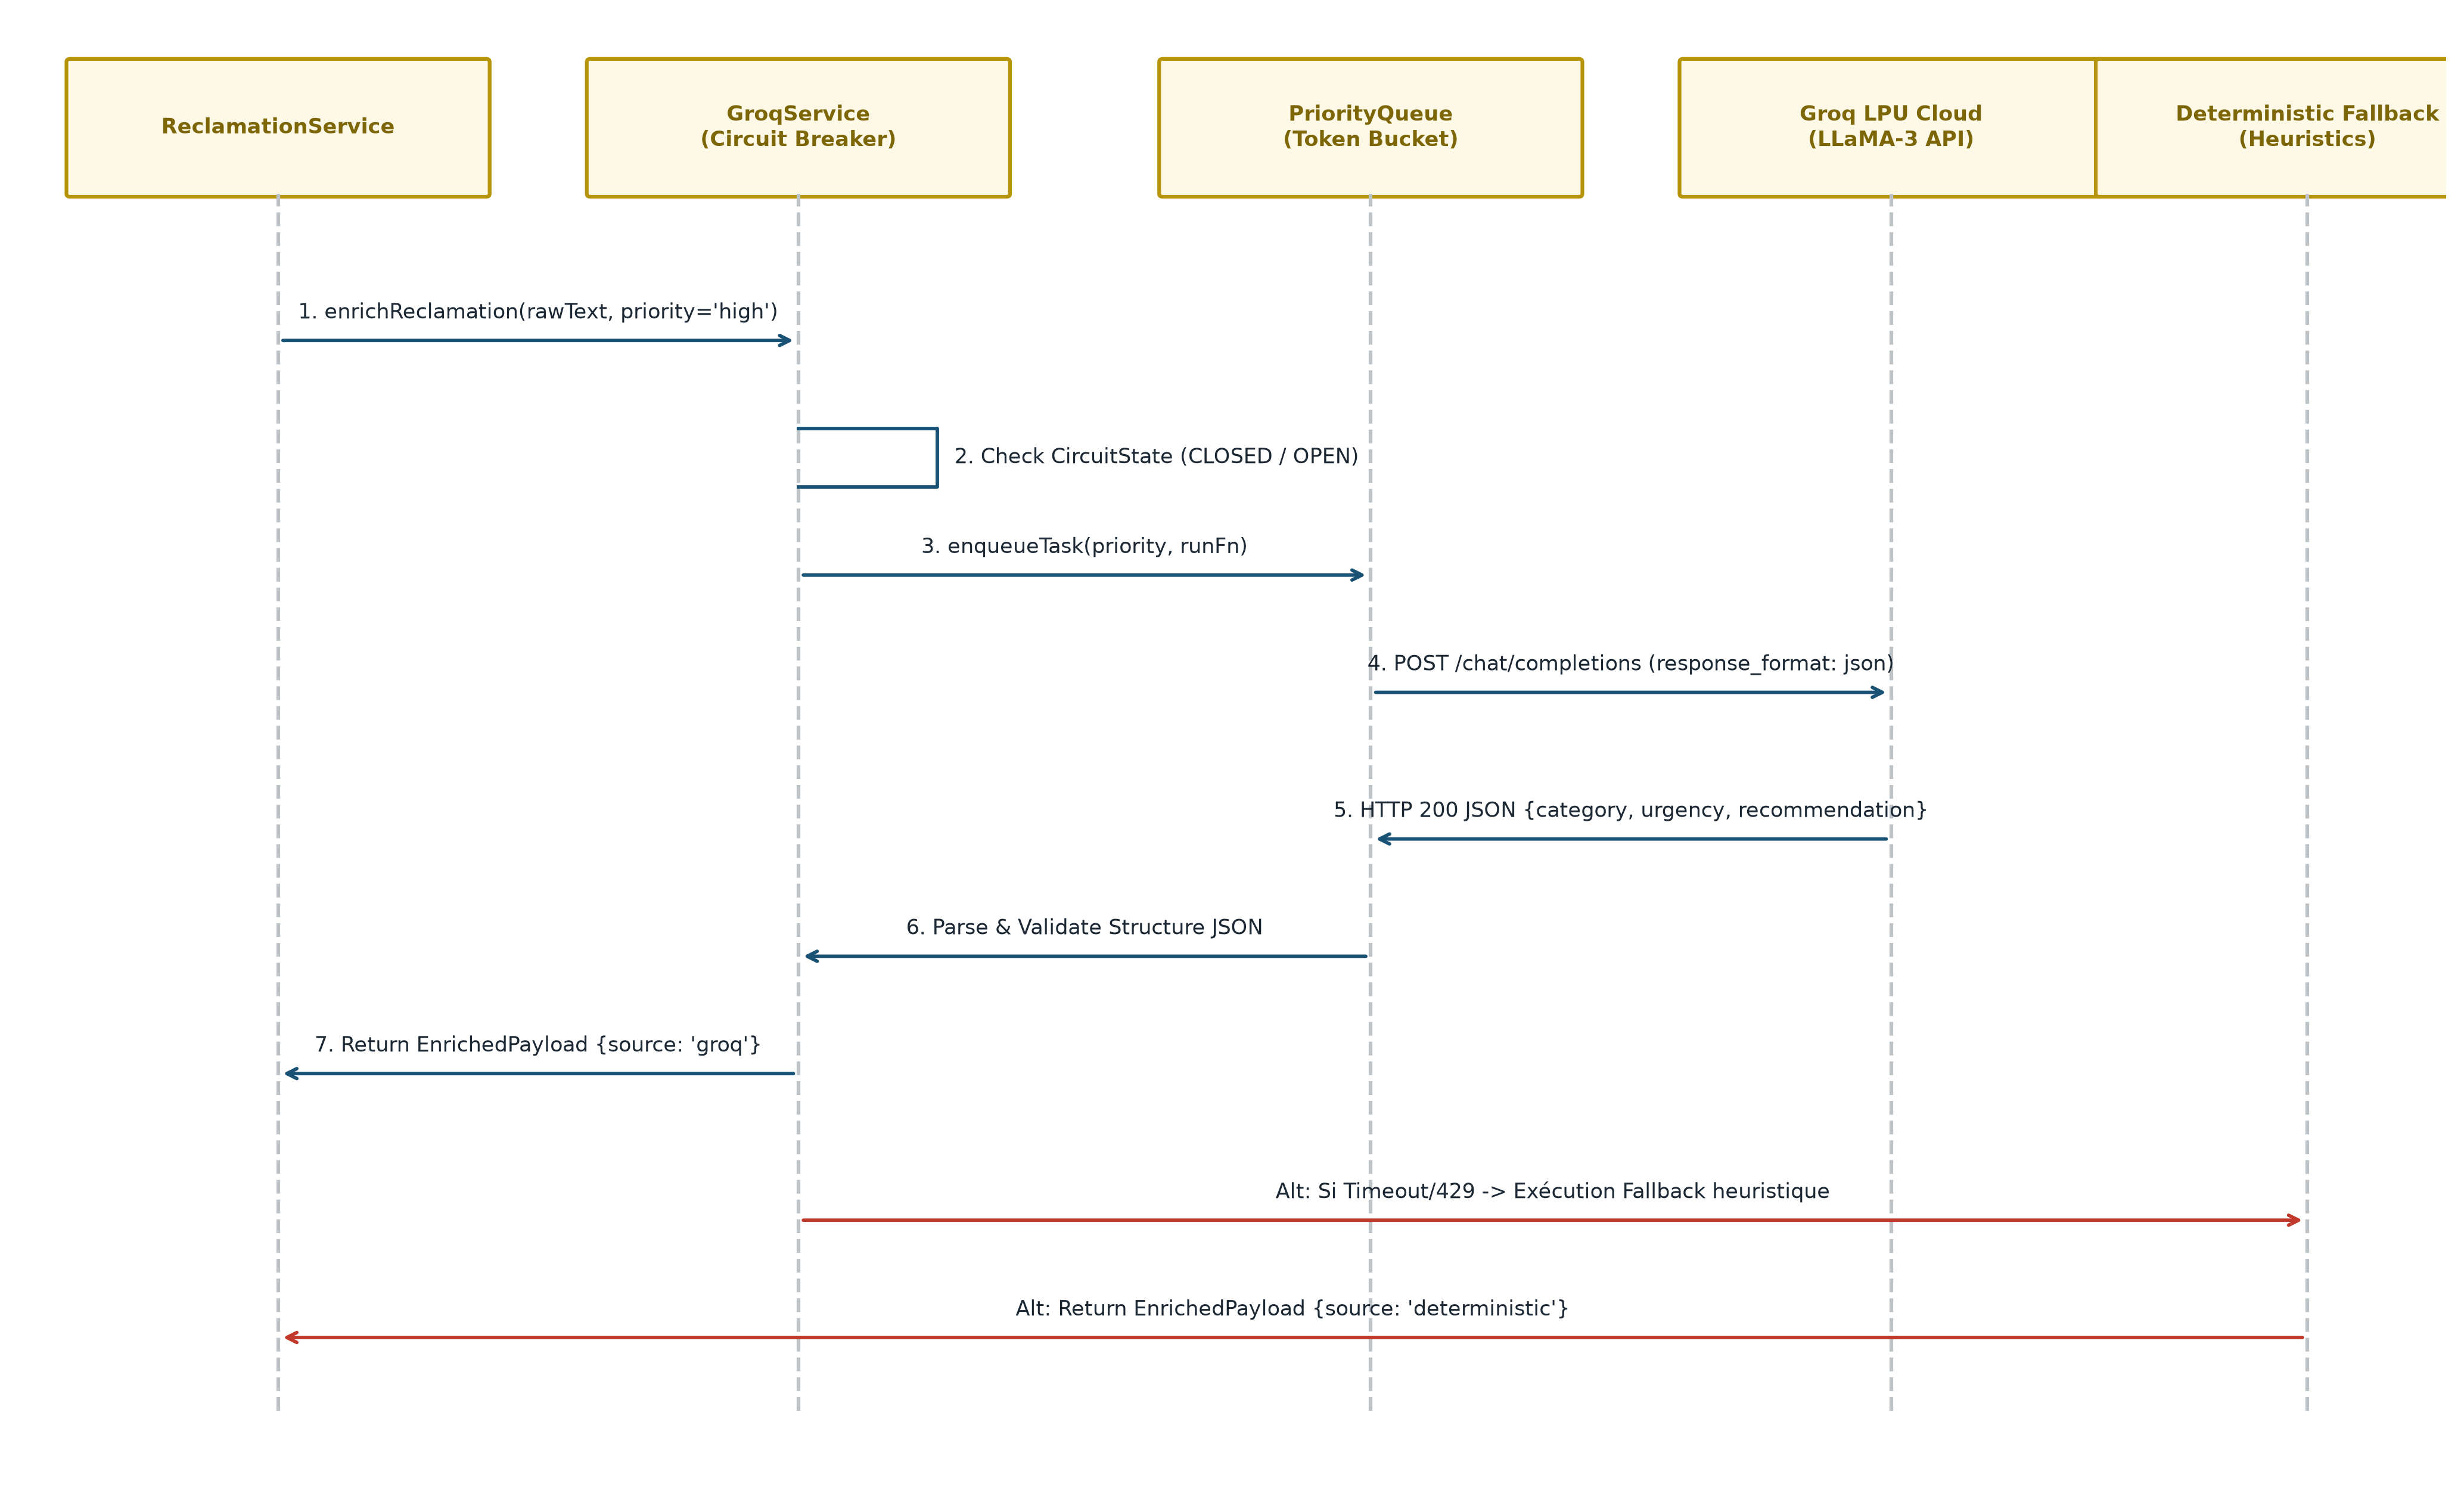
\includegraphics[width=15cm]{Images/ch5/ai_reclamations_sequence.png}
 \caption{Diagramme de s\'equence -- Traitement r\'esilient d'une r\'eclamation par le module IA}
 \label{fig:ch5-ai-seq}
\end{figure}

\section{Strat\'egie de validation et tests logiciels}
Pour garantir la fiabilit\'e et la qualit\'e du code, nous avons mis en \oe uvre une strat\'egie de tests multi-niveaux :
\begin{itemize}
    \item \textbf{Tests Unitaires (Jest / Flutter Test) :} Validation individuelle des m\'ethodes m\'etier, des validateurs DTO, des fonctions de calcul de saturation et des r\'educteurs d'\'etat Riverpod.
    \item \textbf{Tests d'Int\'egration (Supertest) :} V\'erification des flux complets entre les contr\^oleurs NestJS, les services, les guards de s\'ecurit\'e et la base de donn\'ees MongoDB de test.
    \item \textbf{Tests de Non-R\'egression :} Validation automatique de la non-alt\'eration des fonctionnalit\'es existantes apr\`es chaque ajout de code.
\end{itemize}

Le tableau~\ref{tab:test-results} r\'esume les r\'esultats de la campagne de tests men\'ee sur la version finale.

\begin{table}[H]
\centering
\begin{tabular}{|p{4.5cm}|c|c|c|}
\hline
\textbf{Suite de Tests} & \textbf{Tests ex\'ecut\'es} & \textbf{Succ\`es} & \textbf{Couverture de code} \\
\hline
Authentification \& RBAC & 24 & 24 ($100\%$) & 92\% \\
\hline
Gestion Topologie \& G\'eospatial & 38 & 38 ($100\%$) & 88\% \\
\hline
Temps R\'eel (Socket.IO Gateway) & 18 & 18 ($100\%$) & 85\% \\
\hline
Moteur IA \& Circuit Breaker & 22 & 22 ($100\%$) & 94\% \\
\hline
Widgets \& Navigation Flutter & 30 & 30 ($100\%$) & 82\% \\
\hline
\end{tabular}
\caption{Bilan synth\'etique de la couverture et des r\'esultats de tests}
\label{tab:test-results}
\end{table}

\section{D\'eploiement physique et architecture de production}

\subsection{Diagramme de d\'eploiement UML}
La figure~\ref{fig:ch5-deployment} mod\'elise l'architecture mat\'erielle et logicielle de d\'eploiement en production.

\begin{figure}[H]
 \centering
 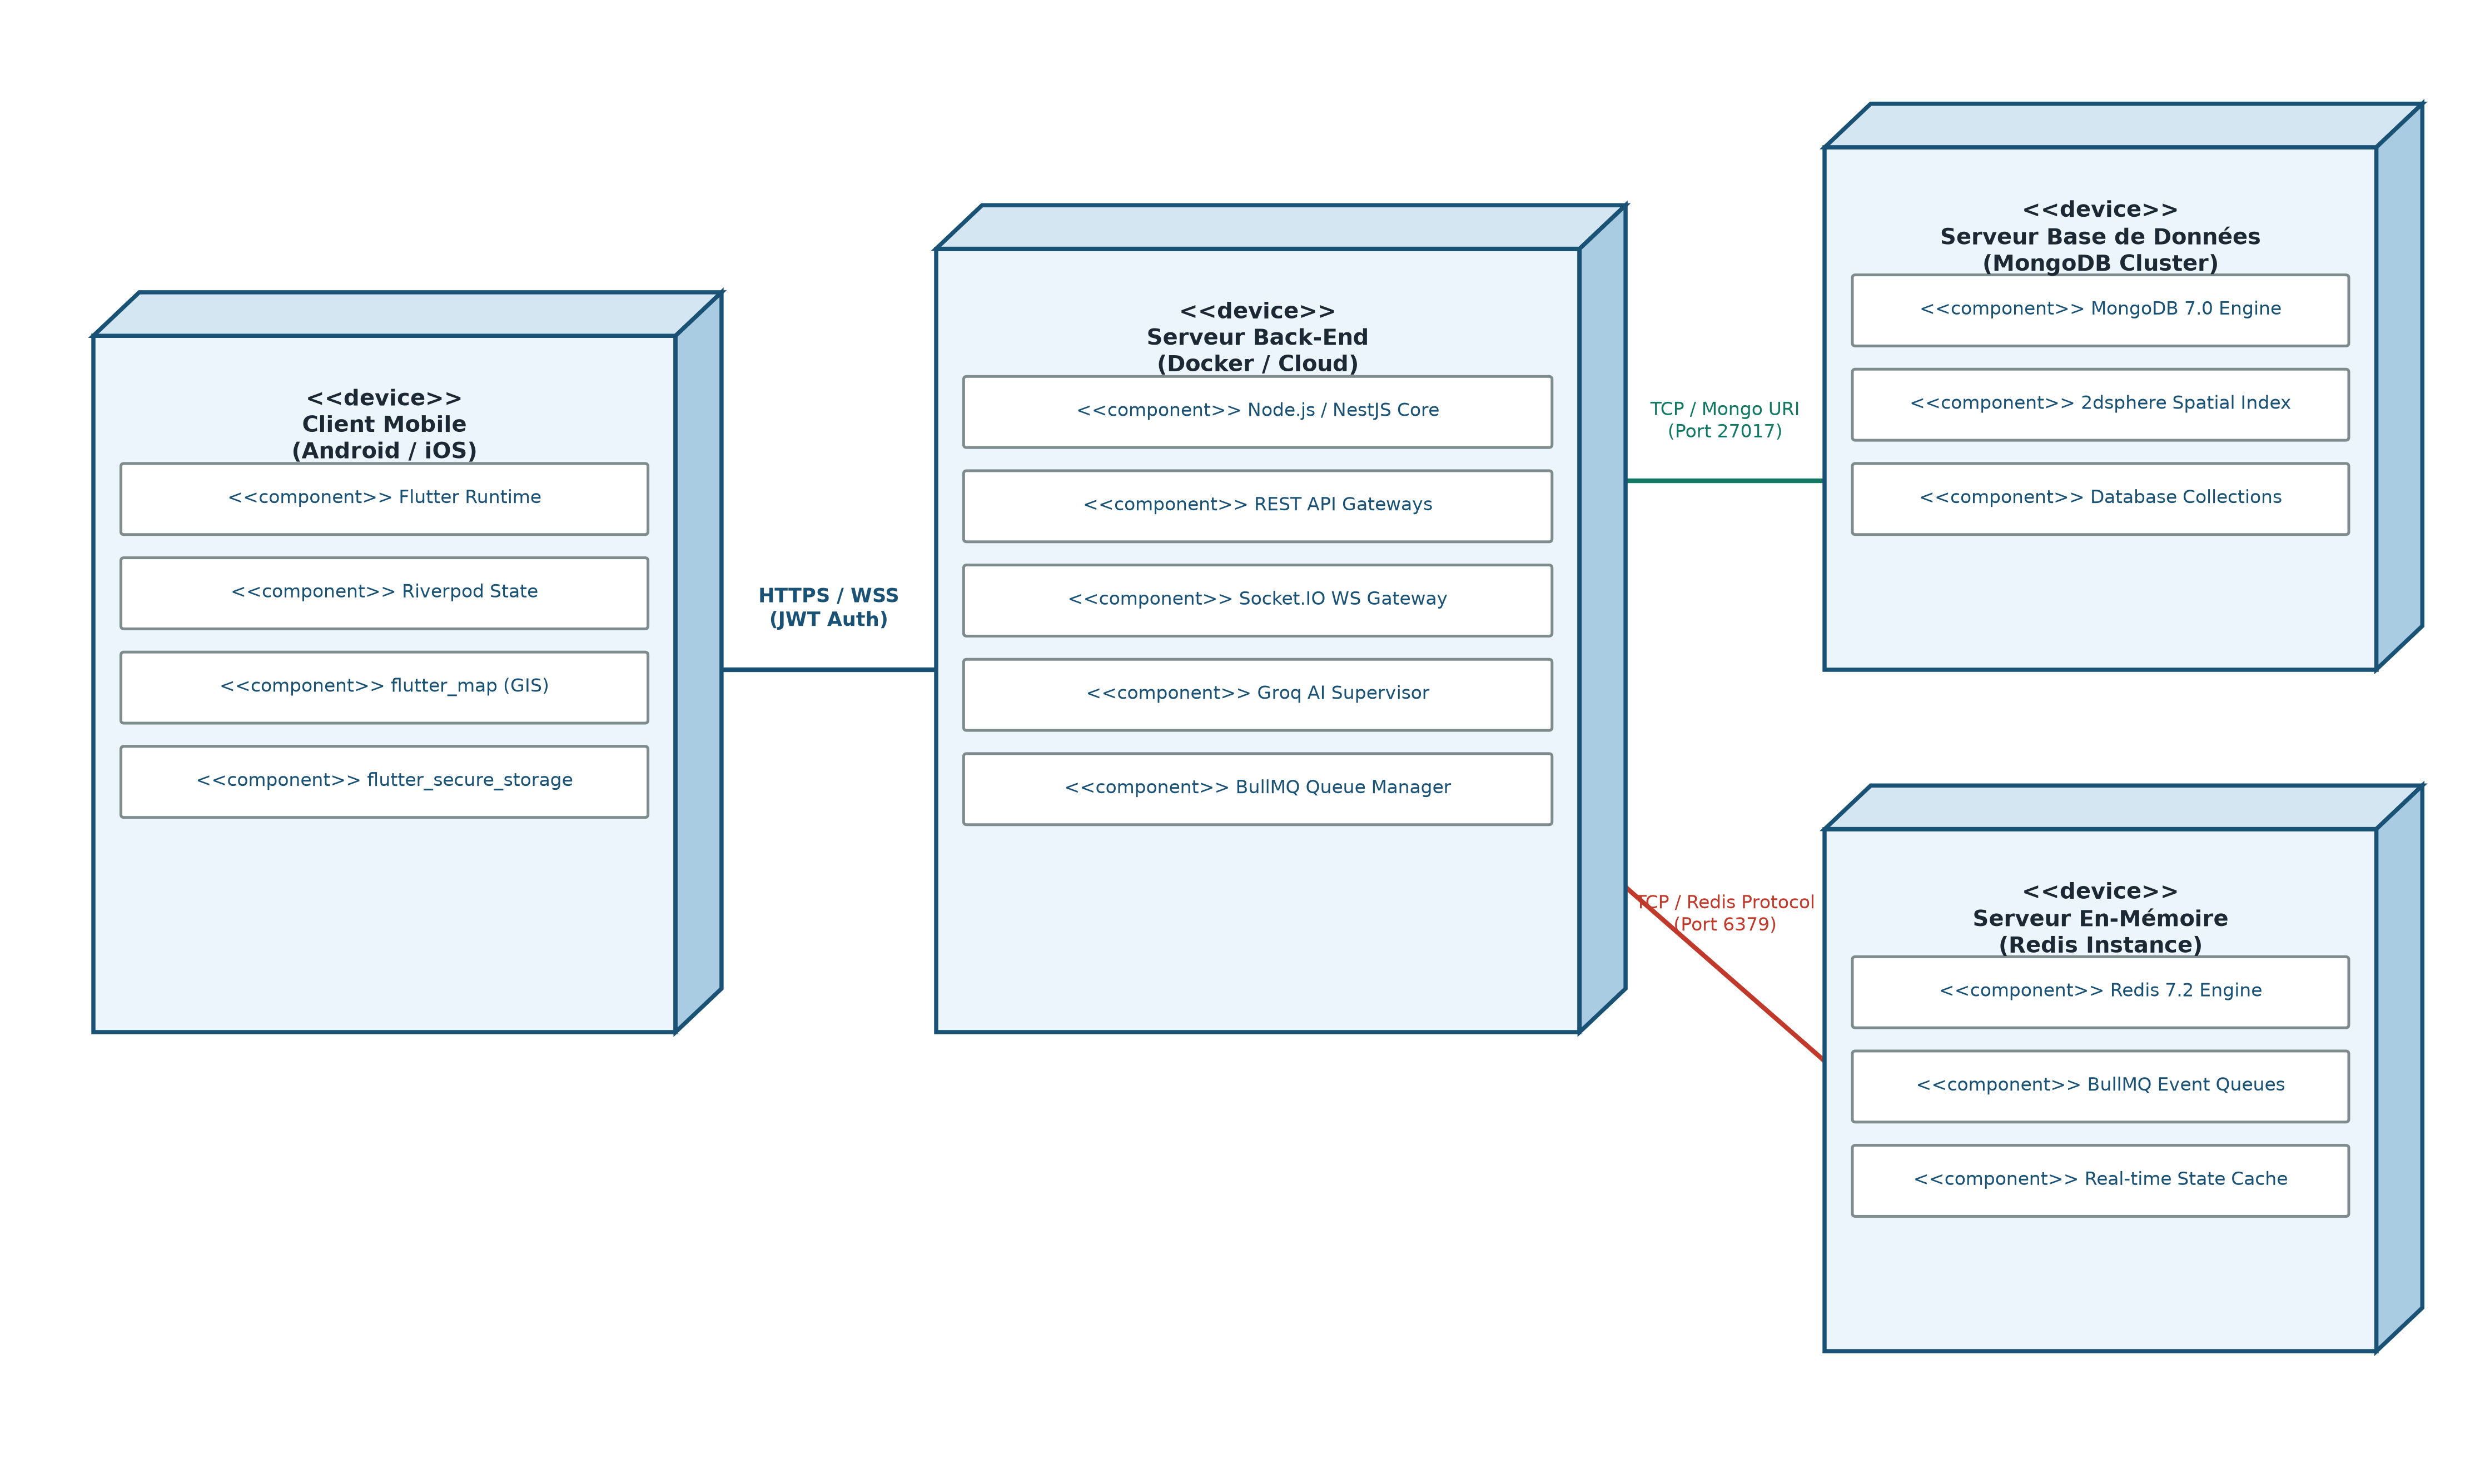
\includegraphics[width=15cm]{Images/ch5/deployment_diagram.png}
 \caption{Diagramme de d\'eploiement UML de la solution globale}
 \label{fig:ch5-deployment}
\end{figure}

L'infrastructure s'organise selon les n\oe uds suivants :
\begin{enumerate}
    \item \textbf{N\oe ud Terminal Mobile (Client) :} Ex\'ecute l'application compil\'ee Flutter (Android APK / iOS IPA), communiquant en HTTPS pour l'API REST et en WSS pour les flux temps r\'eel.
    \item \textbf{N\oe ud Serveur d'Application (NestJS Cluster) :} Conteneur Docker h\'eberg\'e dans un environnement Cloud (Vercel / Serveur Linux), ex\'ecutant l'API Node.js et g\'erant la passerelle Socket.IO.
    \item \textbf{N\oe ud Persistance (MongoDB Cluster) :} Instance de base de donn\'ees avec r\'eplication, s\'ecuris\'ee et isol\'ee dans un r\'eseau priv\'e.
    \item \textbf{N\oe ud Cache \& Files (Redis Instance) :} Moteur m\'emoire d\'edi\'e aux files d'attente BullMQ et \`a la gestion de charge.
    \item \textbf{N\oe ud Tiers (Groq AI Cloud) :} Fournisseur d'API d'inf\'erence LLM externe consomm\'e de mani\`ere s\'ecuris\'ee via cl\'e d'API chiffr\'ee.
\end{enumerate}

\section{Interfaces r\'ealis\'ees pour la Release 3}

\subsection{Visualisation de l'enrichissement IA des r\'eclamations}
La figure~\ref{fig:ch5-ui-ai-rec} illustre l'interface mobile affichant les d\'etails d'une r\'eclamation enrichie automatiquement avec sa cat\'egorie, son niveau d'urgence et la synth\`ese d'action propos\'ee.

\begin{figure}[H]
 \centering
 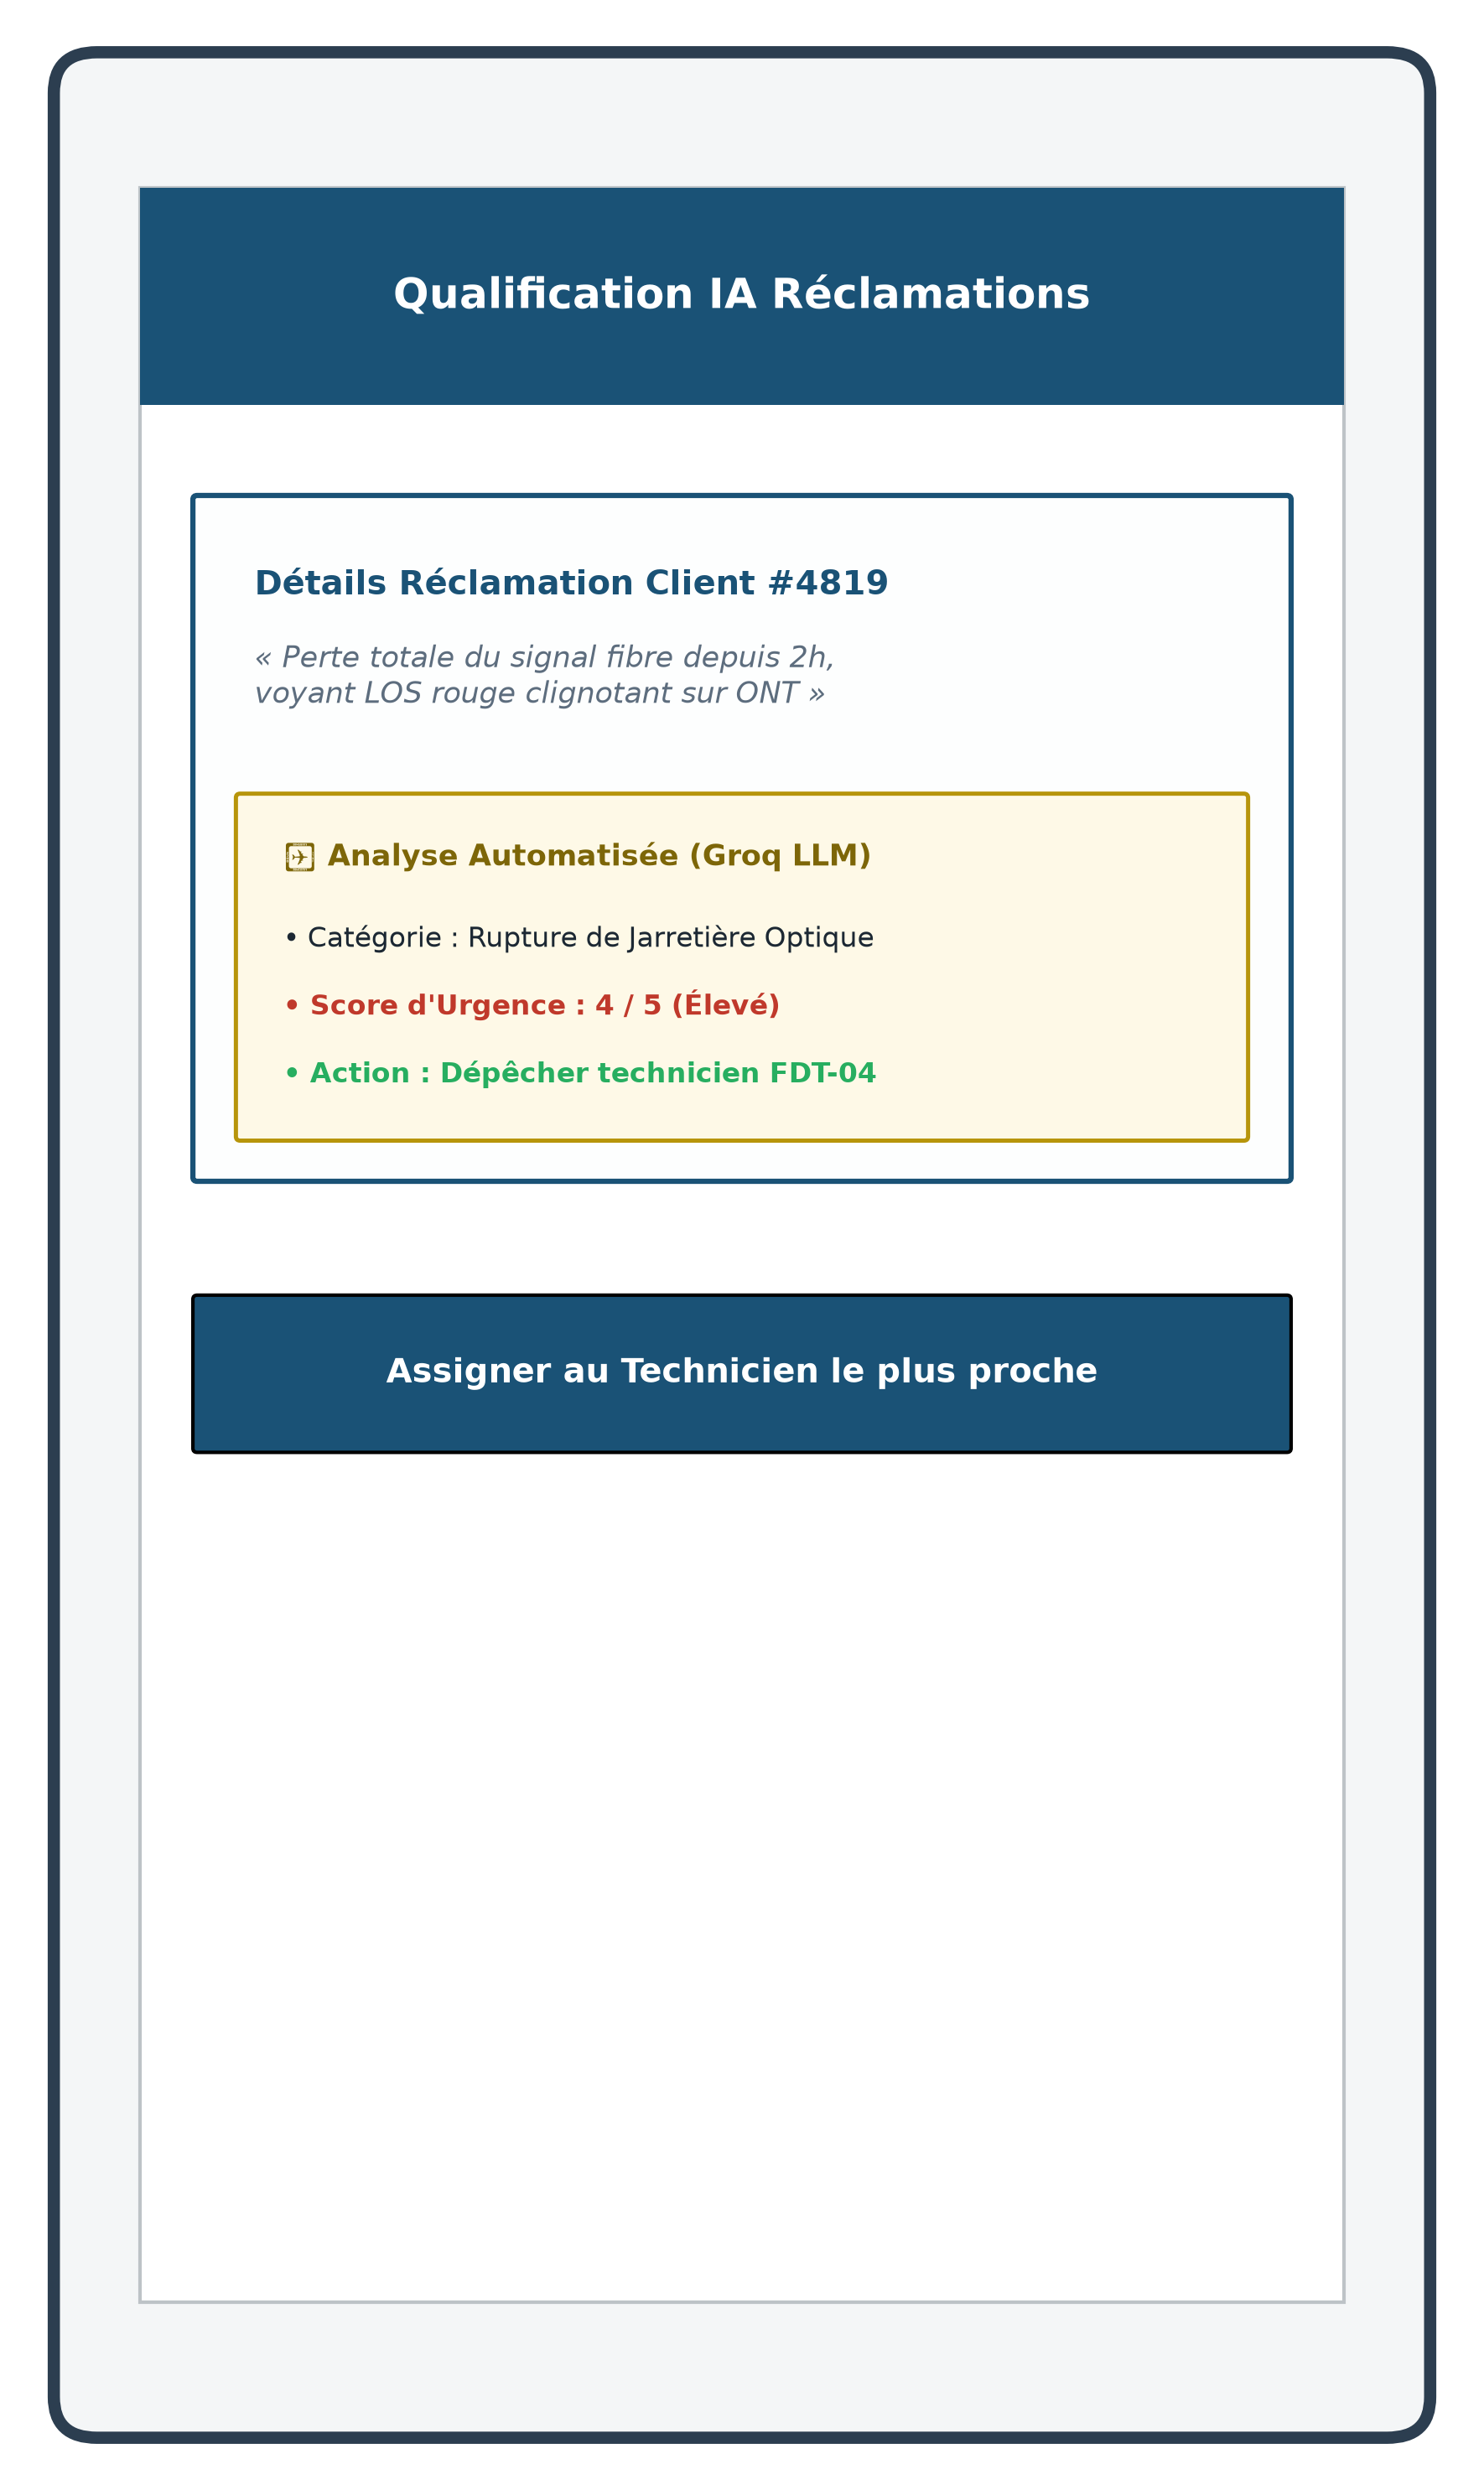
\includegraphics[width=11cm]{Images/ch5/ui_ai_reclamations.png}
 \caption{Interface de restitution de l'enrichissement IA d'une r\'eclamation}
 \label{fig:ch5-ui-ai-rec}
\end{figure}

\subsection{Indicateurs pr\'eventifs de saturation NRO}
La figure~\ref{fig:ch5-ui-ai-sat} montre la vue analytique mettant en \'evidence les NRO \`a risque de saturation imminente.

\begin{figure}[H]
 \centering
 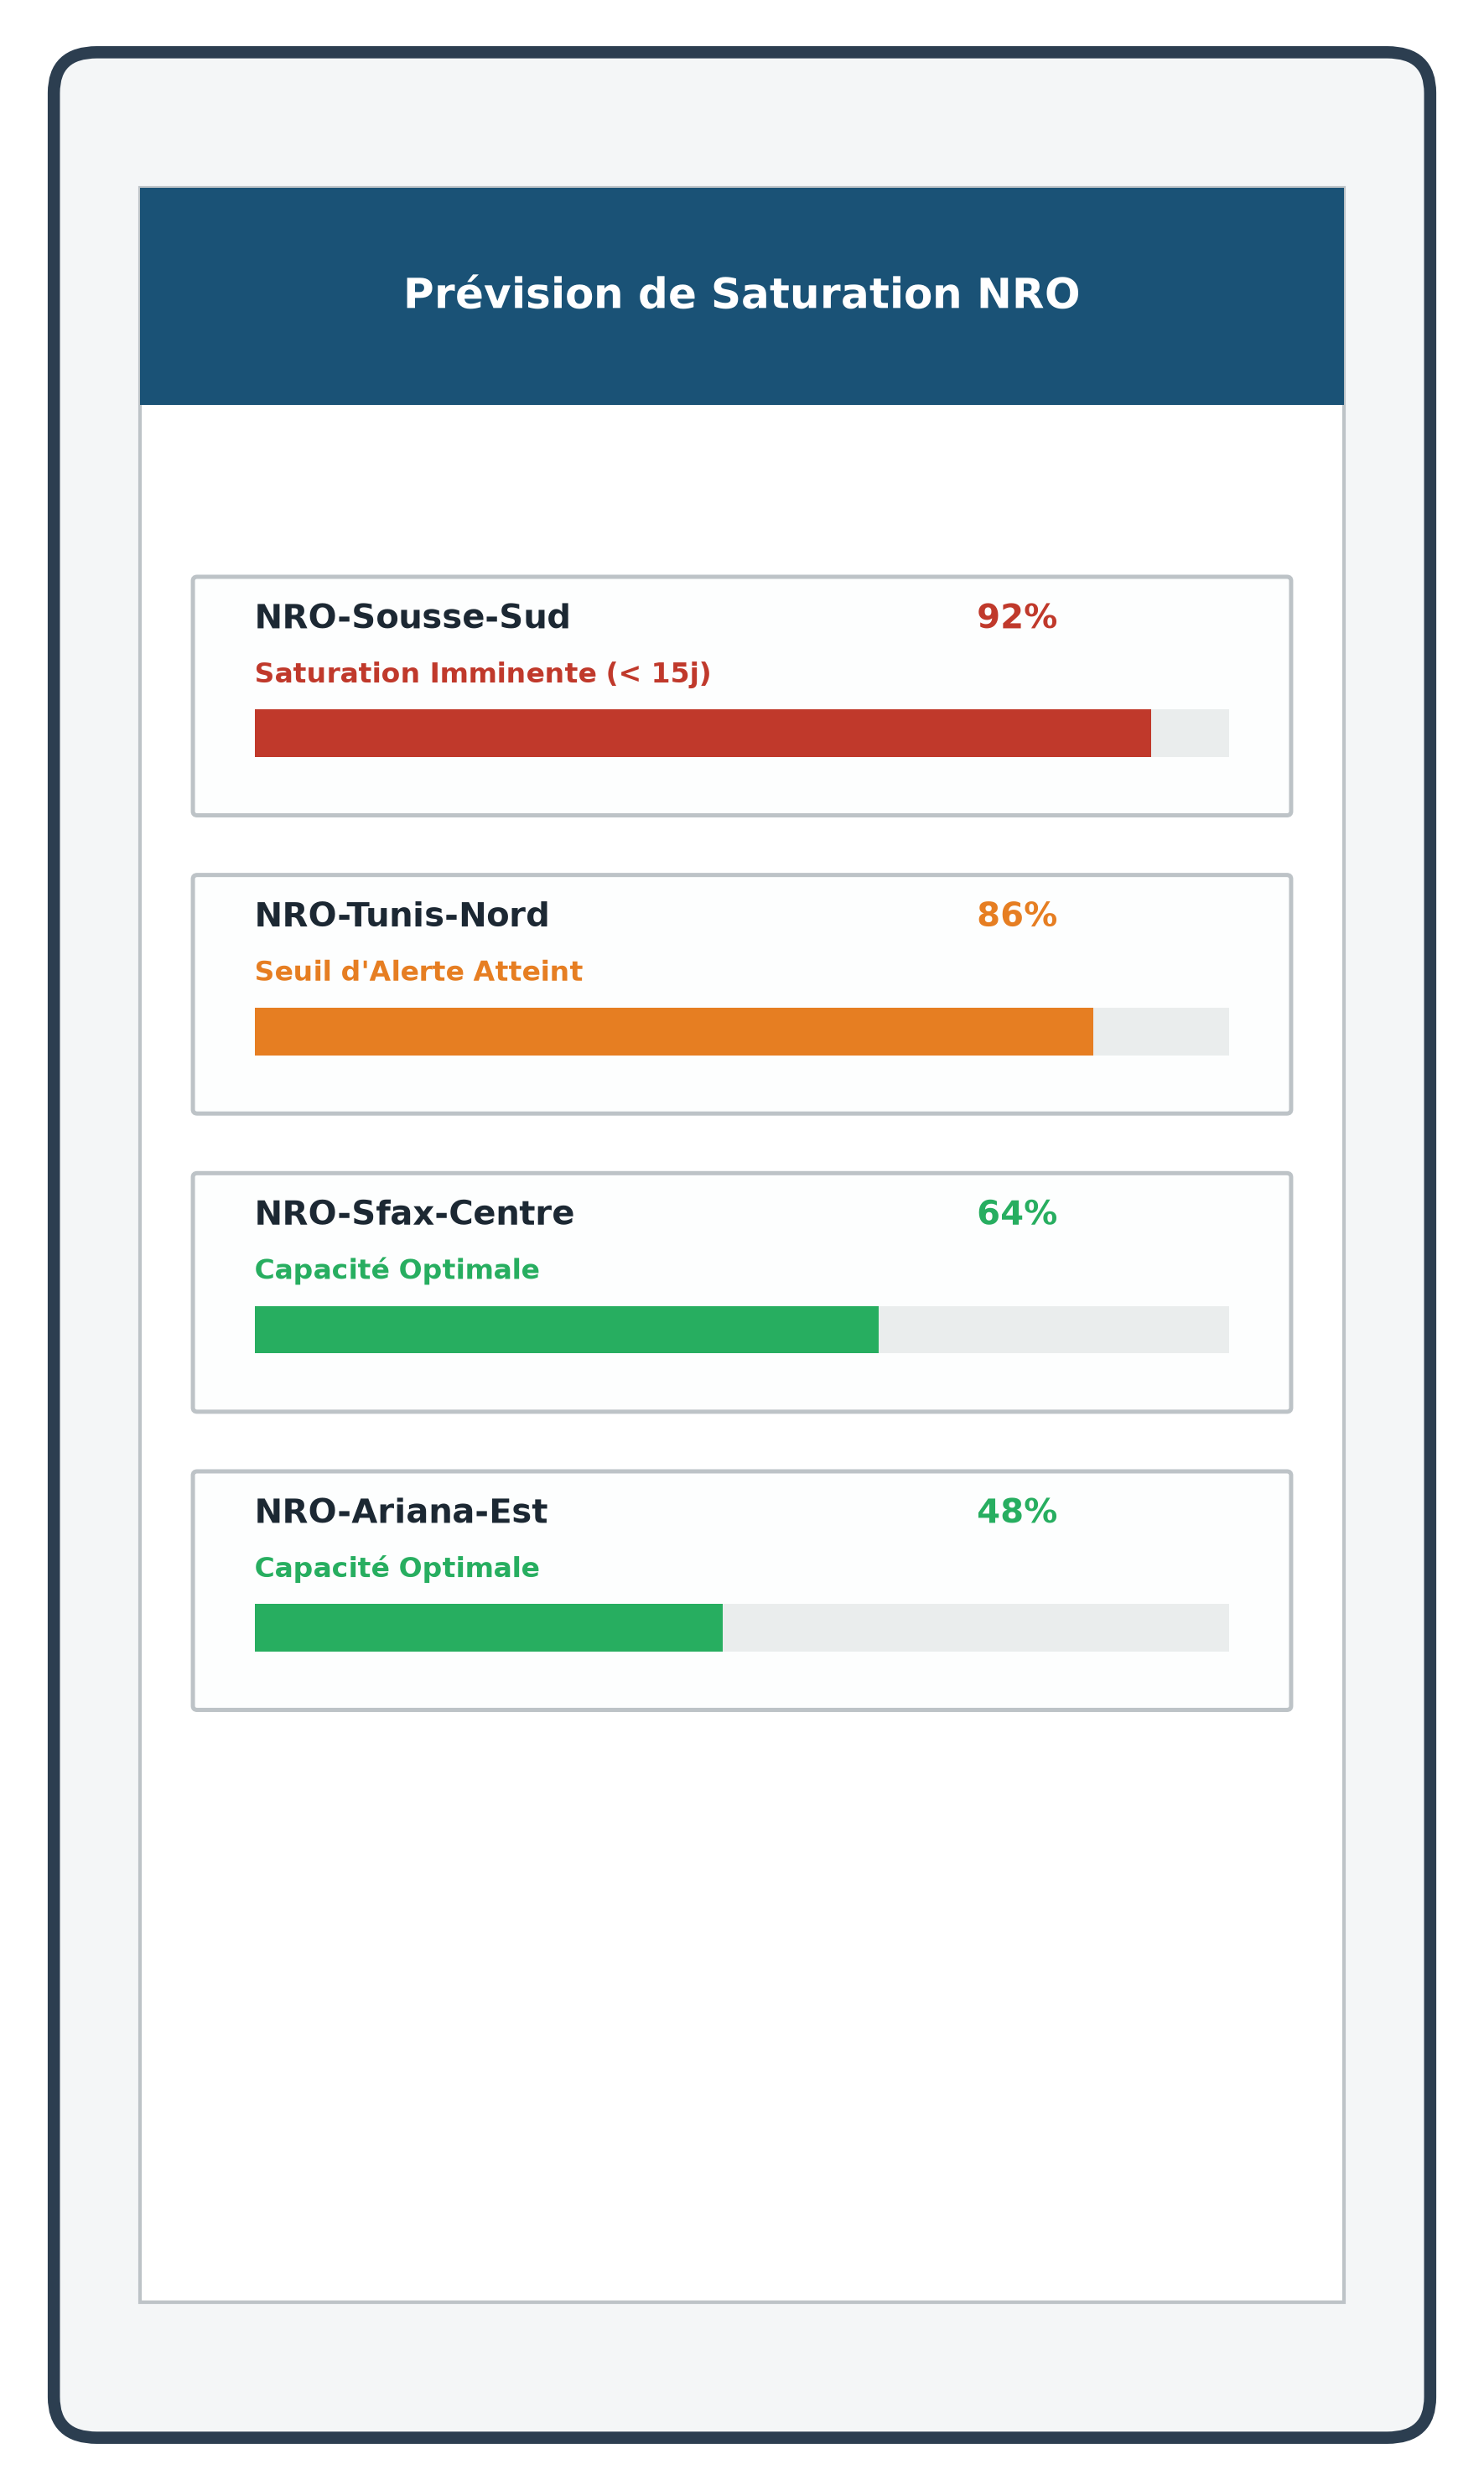
\includegraphics[width=11cm]{Images/ch5/ui_ai_saturation.png}
 \caption{Interface de suivi pr\'edictif de saturation des NRO}
 \label{fig:ch5-ui-ai-sat}
\end{figure}

\section*{Conclusion}
Cette derni\`ere release a consolid\'e l'ensemble des modules de la plateforme en y apportant une v\'eritable valeur d'aide \`a la d\'ecision gr\^ace \`a l'IA, tout en garantissant une haute disponibilit\'e gr\^ace aux m\'ecanismes de r\'esilience. La campagne de tests et la mod\'elisation du d\'eploiement assurent la conformit\'e de la solution aux exigences industrielles de Tunisie Telecom.
